% 第4章第5节：交换序列（交换性、与独立和平稳的比较、de Finetti表示）。

\section{交换序列}
\label{sec:spp-exchangeable}

前几节的依赖大多来自时间：下一步依赖过去，相邻读数共享增量。但第~\ref{sec:spp-index-state-space}小节的共享背景读数提示了另一种来源：所有观测共同受一个随机背景影响，彼此之间并没有先后作用。Pólya罐的路径概率只依赖$1$的个数（示例~\ref{ex:spp-polya-path}），也是这种结构的表现。本节研究观测编号重排后联合规律不变的序列。我们先比较交换性与独立、与时间平移不变性各约束什么，再说明无限交换序列总可以写成“先抽随机背景，再条件独立抽样”，并解释这为什么使经验平均趋向一个随机的极限。

\subsection{交换性与共享随机背景}
\label{sec:spp-exchangeability}

\paragraph{共享成功率的抛掷}
设想一批硬币来自同一台冲压机，每枚的正面概率都是同一个未知值。把这个未知值建模为随机变量$\Theta\sim\operatorname{Beta}(2,2)$，给定$\Theta$后，各次抛掷$X_1,X_2,\ldots$独立服从$\operatorname{Bernoulli}(\Theta)$。对任一含$k$个$1$的序列$(x_1,\ldots,x_n)$，先对给定$\Theta$的条件概率求积，再对$\Theta$平均：
\[
  \mathbb P(X_1=x_1,\ldots,X_n=x_n)=\mathbb E\bigl[\Theta^k(1-\Theta)^{n-k}\bigr].
\]
右边只依赖$k$，不依赖$1$出现在哪些位置。这是本节的核心现象：观测之间相关，但没有哪个编号是特殊的。

相关性可以直接算出。$\Theta\sim\operatorname{Beta}(2,2)$的均值为$1/2$，方差为$1/20$。对$i\ne j$，由塔式性质，
\begin{gather*}
  \mathbb P(X_i=X_j=1)=\mathbb E\Theta^2=\frac1{20}+\frac14=0.3,\\
  \operatorname{Cov}(X_i,X_j)=\mathbb E\Theta^2-(\mathbb E\Theta)^2=\operatorname{Var}(\Theta)=\frac1{20}.
\end{gather*}
两次都是正面的概率$0.3$大于独立时的$0.25$：观测到一次正面，使“这批硬币偏向正面”更可信，从而提高了下一次正面的概率。成功次数$S_n=X_1+\cdots+X_n$的方差也随之增大。由条件方差分解，
\[
  \begin{aligned}
  \operatorname{Var}(S_n)&=\mathbb E\operatorname{Var}(S_n\mid\Theta)+\operatorname{Var}\mathbb E(S_n\mid\Theta)\\
  &=n\,\mathbb E[\Theta(1-\Theta)]+n^2\operatorname{Var}(\Theta)=\frac n5+\frac{n^2}{20},
  \end{aligned}
\]
其中$\mathbb E[\Theta(1-\Theta)]=\frac12-0.3=0.2$。$n=10$时为$7$，而独立$\operatorname{Bernoulli}(1/2)$的成功次数方差只有$2.5$。图~\ref{fig:spp-beta-binomial}比较了两种分布：共享成功率时，极端的成功次数明显更常见。

\begin{figure}[htbp]
  \centering
  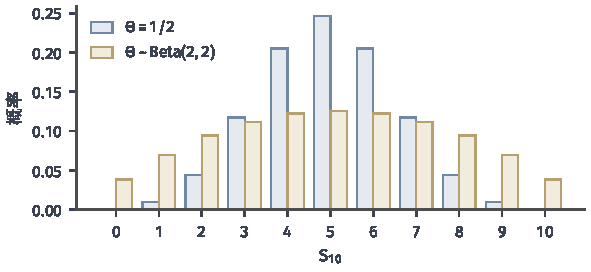
\includegraphics[width=100mm]{figures/03-optimization-evolution-and-signals/02-processes-and-trajectory-evolution/matplotlib/spp-beta-binomial/figure.pdf}
  \caption{十次抛掷中成功次数$S_{10}$的分布（精确概率）。蓝色：成功率固定为$1/2$，各次独立，$S_{10}\sim\operatorname{Bin}(10,1/2)$，方差$2.5$。黄色：成功率$\Theta\sim\operatorname{Beta}(2,2)$由各次共享，给定$\Theta$后独立，方差$7$。两者单次成功概率都是$1/2$。}
  \label{fig:spp-beta-binomial}
\end{figure}

\paragraph{交换性的定义}
把“编号不特殊”写成联合规律的对称性，得到下面的定义。

\begin{definition}[可交换序列]
\label{def:spp-exchangeable}
随机变量$X_1,\ldots,X_n$称为\term{可交换}（exchangeable）的，若对$\{1,\ldots,n\}$的每个排列$\pi$都有
\[
  (X_{\pi(1)},\ldots,X_{\pi(n)})\overset{\mathrm d}{=}(X_1,\ldots,X_n).
\]
无限序列$(X_n)_{n\ge1}$称为可交换的，若对每个$n$，$(X_1,\ldots,X_n)$可交换。这一性质称为\term{交换性}（exchangeability）。
\end{definition}

无限序列的定义等价于：只改变有限个编号的任意排列都不改变整个序列的规律，因为这样的排列只涉及某个前缀，而序列的规律由有限维分布决定。由定义，可交换序列的各项同分布，任意两项的联合分布都相同，任意$m$项的联合分布也只依赖$m$。

\paragraph{交换与独立各约束什么}
交换性与独立性约束联合规律的不同方面。独立同分布序列可交换，因为其联合分布是同一边缘分布的乘积，重排因子不改变乘积。反之，上面的共享成功率序列可交换却不独立；而独立但分布不同的序列，例如$X_i\sim\mathcal N(i,1)$相互独立，则独立却不可交换。独立性说的是联合规律能否分解为乘积，交换性说的是联合规律在重排下是否对称。

交换性对相关系数有一个简单的约束。设$X_1,\ldots,X_n$可交换，方差$\sigma^2>0$，任意两项的相关系数都是$\rho$。则
\[
  0\le\operatorname{Var}\Bigl(\sum_{i=1}^nX_i\Bigr)=n\sigma^2+n(n-1)\rho\sigma^2=n\sigma^2\bigl(1+(n-1)\rho\bigr),
\]
所以$\rho\ge-1/(n-1)$。对无限可交换序列，这对每个$n$都成立，令$n\to\infty$得$\rho\ge0$。负相关只能出现在有限长的可交换序列中。

\begin{example}[不放回抽取]
\label{ex:spp-without-replacement}
罐中有一个$1$球和一个$0$球，不放回地依次摸出，记标号为$X_1,X_2$。$(X_1,X_2)$等概率地取$(1,0)$或$(0,1)$，重排后分布不变，所以可交换。但$\operatorname{Cov}(X_1,X_2)=0-\frac14=-\frac14$，$\operatorname{Var}(X_i)=\frac14$，相关系数为$-1<-\frac12$。由上面的约束，它不能延长为三个可交换变量，更不能延长为无限可交换序列。它也不能写成“先抽$\Theta$、再条件独立抽样”的形式，因为那样得到的任意两项协方差都等于$\operatorname{Var}(\Theta)\ge0$。更一般地，从$N$个球中不放回抽样得到的有限序列可交换，相关系数为$-1/(N-1)$。
\end{example}

\paragraph{交换性与平移不变性}
时间序列中常见的另一种对称性是平移不变性：若对每个$k\ge0$，$(X_{1+k},X_{2+k},\ldots)$与$(X_1,X_2,\ldots)$同分布，就称序列具有\term{严格平稳性}（strict stationarity），简称平稳。无限可交换序列一定平稳：对固定的$n$和$k$，存在$\{1,\ldots,n+k\}$的一个排列把$(1+k,\ldots,n+k)$移到$(1,\ldots,n)$，由交换性，$(X_{1+k},\ldots,X_{n+k})\overset{\mathrm d}{=}(X_1,\ldots,X_n)$，再由有限维分布决定规律即得。

反之不成立。第~\ref{sec:spp-fdd-path-law}小节的平稳自回归序列（$\rho=0.8$）平移不变，但$\operatorname{Corr}(Y_1,Y_2)=0.8$，$\operatorname{Corr}(Y_1,Y_3)=0.64$；若它可交换，交换第$2$、$3$项不改变规律，就应有$(Y_1,Y_2)\overset{\mathrm d}{=}(Y_1,Y_3)$，两个相关系数必须相等。平稳只要求依赖结构不随整体平移改变，允许远近不同的项依赖强弱不同；交换性要求所有项两两地位相同。两种对称性服务于不同的目的：平稳性用于研究长时间平均（第~\ref{chap:discrete-time-stochastic-processes}章的遍历理论），交换性用于描述顺序无关的抽样和由此得到的置换论证。

\subsection{条件独立混合表示}
\label{sec:spp-de-finetti}

\paragraph{频率的极限是随机的}
图~\ref{fig:spp-polya-frequencies}比较了两类序列的累计频率$\bar X_n=S_n/n$。独立的$\operatorname{Bernoulli}(1/2)$序列中，二十条频率曲线都向$1/2$收拢，这是强大数律。Pólya罐（$a=b=1$）的二十条曲线也各自稳定下来，却停在不同的高度；把四千个罐运行两千步，最终频率的直方图几乎是平的。看起来，每个罐在开头几步的偶然结果中“选定”了一个自己的成功率，此后的观测就像以这个成功率独立抽样。

\begin{figure*}[htbp]
  \centering
  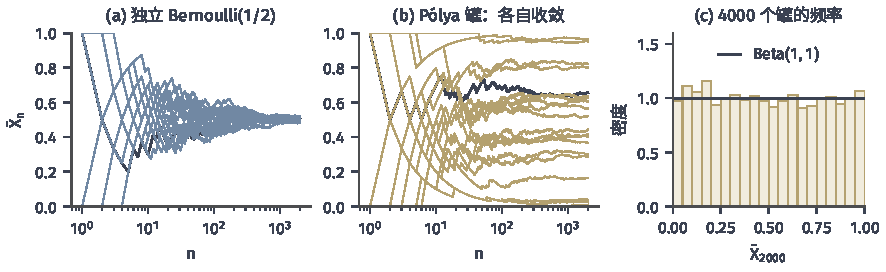
\includegraphics[width=150mm]{figures/03-optimization-evolution-and-signals/02-processes-and-trajectory-evolution/matplotlib/spp-polya-frequencies/figure.pdf}
  \caption{累计频率$\bar X_n=S_n/n$随$n$的变化（横轴为对数刻度）。(a)$20$条独立$\operatorname{Bernoulli}(1/2)$序列，频率都收敛到$1/2$；(b)$20$个Pólya罐（起初一个$1$球、一个$0$球，每次放回并加入一个同色球），频率各自收敛到不同的值；(c)$4000$个Pólya罐在$n=2000$时的频率直方图，黑线为$\operatorname{Beta}(1,1)$即均匀分布的密度。各图中深色曲线标出一条代表路径，随机数使用固定种子。}
  \label{fig:spp-polya-frequencies}
\end{figure*}

这个“自己的成功率”对实值观测而言是一个数，对一般状态空间中的观测而言则是一整个分布：给定背景后，观测独立地服从某个随机选出的概率测度。这样的对象称为\term{随机概率测度}（random probability measure）：它的每次实现是$E$上的一个概率测度，并且对每个可测集$A$，它给$A$的质量是一个随机变量。第~\ref{sec:spp-random-mass}小节将给出准确的可测性定义并研究构造，这里只需要上述两点。

\paragraph{de Finetti定理}
下面的定理说明，图中的现象对一切无限可交换序列都成立。

\begin{theorem}[de Finetti定理]
\label{thm:spp-de-finetti}
设$(E,\mathcal E)$是标准Borel空间，$(X_n)_{n\ge1}$是取值于$E$的无限可交换序列。则存在随机概率测度$\Xi$，它是$(X_n)$的可测函数，使对每个$n$和$A_1,\ldots,A_n\in\mathcal E$，
\[
  \mathbb P(X_1\in A_1,\ldots,X_n\in A_n\mid\Xi)=\prod_{i=1}^n\Xi(A_i)\qquad\text{几乎必然成立};
\]
即给定$\Xi$后，$X_1,X_2,\ldots$条件独立同分布，条件分布为$\Xi$。并且对每个$A\in\mathcal E$，经验频率$\frac1n\sum_{i=1}^n\mathbb I_A(X_i)$几乎必然收敛到$\Xi(A)$。反之，任何具有这种条件独立同分布结构的序列都可交换。
\end{theorem}

这一表示定理的完整证明可参考文献\scite{math-kallenberg2021probability}。

这一结论称为\term{de Finetti定理}（de Finetti theorem）。反向的结论直接可得：给定$\Xi$时，条件概率$\prod_i\Xi(A_i)$在重排$A_i$时不变，取期望后联合规律也不变。等价地，若$Q$为$\Xi$的分布，序列的规律是混合$\int\nu^{\otimes\mathbb N}\,Q(\mathrm d\nu)$：先按$Q$抽一个分布$\nu$，再从$\nu$独立抽样。定理的要求是“无限”可交换：示例~\ref{ex:spp-without-replacement}的有限序列没有这种表示。

\paragraph{Bernoulli情形的证明}
一般情形的证明需要逆向鞅等工具，这里对取值于$\{0,1\}$的序列给出完整证明，它展示了随机背景是怎样从序列本身中“读出来”的。此时随机概率测度由一个数$\Theta=\Xi(\{1\})$决定。

\begin{proof}[$E=\{0,1\}$时的证明]
第一步，路径概率只依赖$1$的个数。由交换性，任意含$k$个$1$、长为$n$的序列有相同的概率，记为$p(n,k)$。因此给定$S_N=X_1+\cdots+X_N=j$时，$(X_1,\ldots,X_N)$在含$j$个$1$的$\binom Nj$种排列上均匀分布。对固定的$n\le N$和固定的长为$n$、含$k$个$1$的模式$\bm x$，前$n$项恰为$\bm x$的条件概率就是不放回抽样的概率：
\[
  \mathbb P\bigl((X_1,\ldots,X_n)=\bm x\bigm|S_N\bigr)=h_N(S_N),
\]
其中
\[
  h_N(j)=\frac{\prod_{i=0}^{k-1}(j-i)\cdot\prod_{l=0}^{n-k-1}(N-j-l)}{\prod_{i=0}^{n-1}(N-i)} .
\]

第二步，频率在$L^2$中收敛。令$p=\mathbb P(X_1=1)$，$q=\mathbb P(X_1=X_2=1)$。由交换性，$\mathbb EX_iX_j=q$对一切$i\ne j$成立。对$M<N$，
\[
  \begin{aligned}
  \mathbb E\Bigl(\frac{S_N}N-\frac{S_M}M\Bigr)^2
  &=\Bigl(\frac pN+\frac{(N-1)q}N\Bigr)+\Bigl(\frac pM+\frac{(M-1)q}M\Bigr)\\
  &\qquad-2\Bigl(\frac pN+\frac{(N-1)q}N\Bigr)\\
  &=(p-q)\Bigl(\frac1M-\frac1N\Bigr),
  \end{aligned}
\]
其中交叉项用了$\mathbb E[S_NS_M]=Mp+(NM-M)q$。右边在$M,N\to\infty$时趋于零，所以$S_N/N$在$L^2$中是Cauchy列，收敛到某个取值于$[0,1]$的随机变量$\Theta$；特别地，$S_N/N$依概率收敛到$\Theta$，$\Theta$是序列的可测函数。

第三步，识别条件分布。把$h_N(j)$写成$n$个比值之积：前$k$个是$(j-i)/(N-i)$，$0\le i<k$；后$n-k$个是$(N-j-l)/(N-k-l)$，$0\le l<n-k$。当$j\ge k$且$N-j\ge n-k$时，每个比值都在$[0,1]$中，且与$j/N$或$1-j/N$相差至多$n/(N-n)$；$n$个取值于$[0,1]$的因子之积，当每个因子改变至多$\delta$时，积改变至多$n\delta$。其余情形下$h_N(j)=0$，而$(j/N)^k(1-j/N)^{n-k}$不超过$n/N$。所以
\[
  \Bigl|h_N(j)-\Bigl(\frac jN\Bigr)^k\Bigl(1-\frac jN\Bigr)^{n-k}\Bigr|\le\frac{n^2}{N-n},\qquad 0\le j\le N .
\]
取$[0,1]$上的有界连续函数$g$。$g(S_N/N)$是$S_N$的函数，由第一步，
\[
  \mathbb E\bigl[\mathbb I_{\{(X_1,\ldots,X_n)=\bm x\}}\,g(S_N/N)\bigr]=\mathbb E\bigl[h_N(S_N)\,g(S_N/N)\bigr].
\]
令$N\to\infty$：左边被积函数依概率收敛到$\mathbb I_{\{(X_1,\ldots,X_n)=\bm x\}}g(\Theta)$，右边由上面的估计依概率收敛到$\Theta^k(1-\Theta)^{n-k}g(\Theta)$，两边都有界，由有界收敛定理得
\[
  \mathbb E\bigl[\mathbb I_{\{(X_1,\ldots,X_n)=\bm x\}}\,g(\Theta)\bigr]=\mathbb E\bigl[\Theta^k(1-\Theta)^{n-k}\,g(\Theta)\bigr].
\]
区间的示性函数可以用一致有界的连续函数逐点逼近，由有界收敛定理，等式对$g$为区间示性函数成立；区间族对有限交封闭并生成Borel $\sigma$代数，再由$\pi$--$\lambda$论证，等式对$g=\mathbb I_B$、$B$为任意Borel集都成立。这正说明$\mathbb P((X_1,\ldots,X_n)=\bm x\mid\Theta)=\Theta^k(1-\Theta)^{n-k}$几乎必然成立：给定$\Theta$，前$n$项条件独立同分布于$\operatorname{Bernoulli}(\Theta)$。

最后，给定$\Theta$后序列条件独立同分布，对条件分布用强大数律，几乎必然有$S_N/N\to\Theta$；这里的$\Theta$与第二步的$L^2$极限几乎必然相同。
\end{proof}

证明的结构值得记住：随机背景$\Theta$不是额外假设的，而是作为频率的极限从序列中构造出来的；给定前$N$项的总数后，前$n$项像是从一个“大罐”中不放回抽取，$N\to\infty$时不放回抽样变成有放回抽样，即条件独立。

\paragraph{Pólya罐的混合律}
de Finetti定理保证Pólya罐有一个随机成功率$\Theta$，路径概率~\eqref{eq:spp-polya-path}还能确定它的分布。对$\Theta\sim\operatorname{Beta}(a,b)$，利用Beta函数与Gamma函数的关系$B(u,v)=\Gamma(u)\Gamma(v)/\Gamma(u+v)$和$\Gamma(c+j)=c^{(j)}\Gamma(c)$，
\[
  \mathbb E\bigl[\Theta^k(1-\Theta)^{n-k}\bigr]=\frac{B(a+k,\,b+n-k)}{B(a,b)}=\frac{a^{(k)}\,b^{(n-k)}}{(a+b)^{(n)}} ,
\]
与式~\eqref{eq:spp-polya-path}完全相同。取$k=n$可知两个$\Theta$的各阶矩一致；$[0,1]$上的分布由各阶矩决定，因为多项式在$C[0,1]$中一致稠密，于是Pólya罐的随机成功率服从$\operatorname{Beta}(a,b)$。$a=b=1$时是均匀分布，与图~\ref{fig:spp-polya-frequencies}(c)的平直直方图一致。一个逐步强化“多数”的罐，与一枚成功率先随机选定、再独立抛掷的硬币，具有完全相同的联合规律。

\paragraph{随机背景与经验平均的极限}
de Finetti表示改变了对“样本平均收敛到什么”的回答。对可交换序列，$\bar X_n$几乎必然收敛，但极限是随机的$\Theta$（一般地是$\Xi$的相应积分），而不是常数$\mathbb EX_1=\mathbb E\Theta$；只要$\Theta$不退化，$\operatorname{Var}(\bar X_n)\to\operatorname{Var}(\Theta)>0$。这与第~\ref{sec:spp-fdd-path-law}小节共享背景序列的平均方差趋于$\rho$是同一现象。给定背景后，独立同分布的全部理论都可以使用；不给定背景时，需要先说明想要估计的是背景本身，还是背景的总体平均。

本节只研究交换序列的联合结构。基于交换性的置换与共形预测、给定观测后对背景的后验更新，以及背景能否由数据识别，都属于统计推断问题，由卷四的统计推断部分处理。
